\documentclass[11pt,a4paper]{article}

% ---------------------------------------------------------------------------
% Certified localization of reaction deletions in autocatalytic networks:
% ranked support witnesses, witness selection, and exact robustness laws.
%
% Author metadata: set the three macros below before submission.
% ---------------------------------------------------------------------------
\newcommand{\PaperAuthor}{Anonymous manuscript}
\newcommand{\PaperAffiliation}{}
\newcommand{\PaperDate}{September 7, 2026}

\usepackage[T1]{fontenc}
\usepackage[utf8]{inputenc}
\usepackage{lmodern}
\usepackage{microtype}
\usepackage[a4paper,margin=1.05in]{geometry}
\usepackage{amsmath,amssymb,amsthm,mathtools}
\usepackage{booktabs}
\usepackage{array}
\usepackage{enumitem}
\usepackage{xcolor}
\usepackage{graphicx}
\usepackage{tikz}
\usetikzlibrary{arrows.meta,positioning,calc,shapes.geometric}
\usepackage{url}
\usepackage[numbers,sort&compress]{natbib}
\usepackage[colorlinks=true,linkcolor=blue!55!black,citecolor=blue!55!black,urlcolor=blue!55!black]{hyperref}

\setlist{itemsep=2pt,topsep=3pt}
\setlength{\emergencystretch}{1.5em}

\theoremstyle{plain}
\newtheorem{theorem}{Theorem}[section]
\newtheorem{proposition}[theorem]{Proposition}
\newtheorem{lemma}[theorem]{Lemma}
\newtheorem{corollary}[theorem]{Corollary}
\theoremstyle{definition}
\newtheorem{definition}[theorem]{Definition}
\newtheorem{example}[theorem]{Example}
\theoremstyle{remark}
\newtheorem{remark}[theorem]{Remark}

\newcommand{\R}{\mathbb{R}}
\newcommand{\N}{\mathbb{N}}
\newcommand{\E}{\mathbb{E}}
\renewcommand{\Pr}{\mathbb{P}}
\newcommand{\cl}{\mathrm{cl}}
\newcommand{\Anc}{\mathrm{Anc}}
\newcommand{\Var}{\mathrm{Var}}
\newcommand{\lean}[1]{\texttt{#1}}
\DeclareMathOperator{\im}{im}

\title{Certified localization of reaction deletions in autocatalytic networks:\\ ranked support witnesses, witness selection, and exact robustness laws}
\author{\PaperAuthor\\ \PaperAffiliation}
\date{\PaperDate}

\begin{document}
\maketitle

\begin{abstract}
A reflexively autocatalytic and food-generated (RAF) set is the standard combinatorial model of a self-sustaining reaction network. We study what happens to the maximum RAF of a finite catalytic reaction system when reactions are deleted, from three directions. First, we introduce \emph{ranked support witnesses}: for every reaction of the baseline maximum RAF, a set of producer parents whose ranks decrease along reactant edges, together with one unrestricted catalytic parent. We prove that the part of the baseline not reachable from a deletion along selected edges survives every deletion, and that the exact new maximum RAF is recovered by one residual computation inside the reachable cone. This localizes any deletion query to a source-checkable region and admits an exact charge-model theorem: on an explicit unbounded family, a packet evaluator beats a specified fresh evaluator by any prescribed constant factor. Second, we ask which witness to store. The reachable cone always contains the true loss, and the excess above that intrinsic floor is the only thing witness selection can change. Every single deletion admits a perfect witness, the true loss equals the intersection of all witness cones, singleton dependence is a preorder, and synergistic loss under combined deletions prevents any one witness from being perfect for every singleton. Weighted selection is exactly separable on a one-layer source class, becomes NP-complete after one downstream aggregator through an exact reduction from set cover, is repaired by portfolios that keep exact answers through a residual solve and admit the classical greedy coverage guarantee, and yet can require $2^{k}$ witnesses for universally exact regions on a source with $2k+1$ reactions although two suffice for all singletons. Third, for independent random deletion we derive exact robustness laws: the first derivative of expected surviving size is the total singleton loss; the second derivative is twice the sum, over pairs, of overlapping singleton damage minus cooperative pair damage; on functional sources with one alternative catalytic site, two forward exposure sets decide survival under every availability set, yield the complete classification of inclusion-minimal external cuts, an exact objective for choosing one catalyst addition, and an exact variance formula whose overlap count is the obstruction to concentration. Disjoint catalytic modules and a common gateway separate size bias from collective criticality and concentration from persistent fluctuations. The finite statements are compiled in Lean~4 against Mathlib with warnings promoted to errors and no admitted proofs; the few hand-proved consequences are listed explicitly. The results concern structural RAF survival, not kinetic persistence.
\end{abstract}

\noindent\textbf{Keywords.} autocatalytic sets; RAF theory; reaction deletion; incremental computation; certificates; set cover; Russo--Margulis formula; robustness; formal verification.

\medskip
\noindent\textbf{MSC 2020.} 92E20, 68Q17, 68Q25, 60C05, 90C27, 68V20.

\section{Introduction}\label{sec:intro}

A catalytic reaction system consists of molecules, reactions with reactant and product sets, a food set of externally supplied molecules, and a relation recording which molecules catalyse which reactions. Kauffman \citep{kauffman1986} proposed that self-sustaining networks of mutually catalytic reactions could emerge in such systems, and Hordijk and Steel \citep{hordijk2004} gave the now standard formalization: a \emph{reflexively autocatalytic and food-generated} (RAF) set is a nonempty set of reactions each of which has all reactants and at least one catalyst in the closure of the food under the set. RAF sets are closed under union, so every availability set of reactions contains a unique maximum RAF, and it is computable in polynomial time by alternating food closure with pruning \citep{hordijk2004,hordijk2015}. RAF theory has been applied to metabolic networks \citep{sousa2015}, to the emergence of autocatalysis in random chemistries \citep{hordijk2017}, and, in its structural and algorithmic aspects, to a growing body of results on generation orderings, irreducible RAFs and residual constructions \citep{steel2020,huson2024}.

This paper is about \emph{reaction deletion}. Given a baseline maximum RAF $S$, deleting a set $K$ of reactions leaves the maximum RAF of $S\setminus K$, and the reactions lost are $L(K)=S\setminus M(S\setminus K)$. Deletion analysis is the basic sensitivity tool of the field: Sousa et al.\ \citep{sousa2015} measured how the \emph{E.~coli} maximum RAF shrinks when individual catalysts or reactions are removed, and essential reactions are a recurring theme in \citep{steel2020,huson2024}. Three questions organize the present work.
\begin{enumerate}[label=(\roman*)]
\item \emph{Localization.} A deletion query can be answered by recomputing the maximum RAF from scratch. Can the recomputation be confined, with an exact answer, to a region determined by a checkable witness derived from the source?
\item \emph{Selection.} Such witnesses are far from unique. Which one should be stored, how hard is the choice, and what does a collection of witnesses buy?
\item \emph{Structure.} Independently of any algorithm, which features of the source determine the damage caused by deletion, in expectation and in fluctuation?
\end{enumerate}
The three questions share one object, the \emph{ranked support witness}, and one semantic contract, the ordinary RAF semantics in which a catalyst need not be present before the reaction it catalyses fires. We answer them in turn with theorems that are, with the exceptions listed in Section~\ref{sec:notformal}, compiled in Lean~4 \citep{demoura2021} against Mathlib \citep{mathlib2020}.

\subsection{Main results}\label{sec:mainresults}

Throughout, $Q$ is a finite catalytic reaction system, $M(A)$ is the maximum RAF contained in $A$ (or $\emptyset$), and $S=M(A_0)$ is a fixed baseline with $n=|S|$.

\paragraph{Certified localization (Section~\ref{sec:localization}).}
A ranked support witness $W=(p,\lambda)$ on $S$ assigns to each reaction $r\in S$ a parent set $p(r)$ and a rank $\lambda(r)\in\N$ such that every nonfood reactant of $r$ is produced by a parent of strictly smaller rank and at least one catalyst of $r$ is food or is produced by a parent of any rank (Definition~\ref{def:witness}). Witnesses exist for every RAF (Lemma~\ref{lem:existence}). Writing $C_W(K)$ for the set of baseline reactions reachable from $K$ along selected parent edges, we prove:
\begin{itemize}
\item \textbf{Retention and residual identity (Theorems~\ref{thm:retention} and~\ref{thm:localization}).} Any subset of $S$ closed under selected parents is a RAF or empty and survives every deletion avoiding it; consequently, for any region $E\supseteq D$ whose complement $O=S\setminus E$ is parent-closed,
\[
M(A_0\setminus D)\;=\;O\,\cup\,M_{Q_O}\big((S\setminus D)\cap E\big),
\]
where $Q_O$ is $Q$ with the products of $O$ adjoined to the food. In particular $L(D)\subseteq C_W(D)$ for every valid $W$.
\item \textbf{Closed-seed shortcut (Proposition~\ref{prop:closedseed}).} If no selected edge leaves $K$, then $L(K)=K$ with no residual computation.
\item \textbf{Charge-model amortization (Theorem~\ref{thm:family}).} On an explicit connected family with $2n+1$ reactions whose stoichiometric columns lie on distinct positive rays, a sequential packet evaluator returns the literal maximum-RAF membership trace and, for any prescribed factor $t$ with $1150\,t\le 2n+1$ and any valid edit sequence longer than an explicit setup cap, its total charge is less than $1/t$ of the charge of a specified fresh evaluator.
\end{itemize}

\paragraph{Witness selection (Section~\ref{sec:selection}).}
For nonnegative singleton weights $w$, the cost of a witness is $J_w(W)=\sum_{d\in S}w_d\,|C_W(\{d\})|$.
\begin{itemize}
\item \textbf{Intrinsic floor and perfect queries (Proposition~\ref{prop:floor}, Theorem~\ref{thm:perfect}).} Expected cone size decomposes as expected actual loss plus expected excess, and only the excess depends on $W$. Every deletion set $K$ admits a witness $W_K$ with $C_{W_K}(K)=L(K)$; hence $L(K)=\bigcap_W C_W(K)$ over all valid witnesses.
\item \textbf{Intrinsic dependence and synergy (Theorems~\ref{thm:preorder} and~\ref{thm:synergy}).} The relation $d\preccurlyeq r\iff r\in L(\{d\})$ is a preorder on $S$. If some deletion set has \emph{synergistic} loss $L(K)\setminus\bigcup_{d\in K}L(\{d\})\neq\emptyset$, no single witness is perfect for every singleton.
\item \textbf{An exactly solvable class and a hardness wall (Theorems~\ref{thm:onelayer}, \ref{thm:setcover}, \ref{thm:npc}).} On a one-layer producer--consumer source class, weighted selection is separable and a minimum-weight rule is globally optimal over all valid witnesses. Adding one downstream aggregator gives an exact equivalence between witness cost thresholds and set cover; the uniform-mean threshold problem for ranked witnesses is NP-complete.
\item \textbf{Portfolios and their limits (Theorems~\ref{thm:portfolio}, \ref{thm:greedy}, \ref{thm:exponential}).} A finite portfolio of witnesses answers every deletion exactly through one residual solve on the intersection of its cones; greedy selection from a finite pool attains the $1-(1-1/b)^{b}$ coverage guarantee on a training workload. Nevertheless there is a food-catalysed source with $2k+1$ reactions on which exact intersection regions for every deletion set require exactly $2^{k}$ witnesses, although two suffice for all singleton deletions.
\end{itemize}

\paragraph{Exact robustness laws (Section~\ref{sec:robustness}).}
Retain each reaction of $S$ independently with probability $p$ and let $\Phi(p)=\E|M(A_p)|$ and $F(p)=\Pr[M(A_p)\neq\emptyset]$.
\begin{itemize}
\item \textbf{First and second order (Proposition~\ref{prop:firstorder}, Theorem~\ref{thm:curvature}).} $\Phi'(1)=\sum_i|L(\{i\})|$, $F'(1)$ counts the singletons whose deletion extinguishes the RAF, and
\[
\Phi''(1)=2\sum_{\{i,j\}\subseteq S}\Big(|L(\{i\})\cap L(\{j\})|-|C_{ij}|\Big),\qquad C_{ij}=L(\{i,j\})\setminus\big(L(\{i\})\cup L(\{j\})\big).
\]
Curvature therefore separates two mechanisms that the mean singleton loss cannot distinguish: overlapping damage, which makes repeated deletions redundant, and cooperative failure, which makes a pair worse than the sum of its parts.
\item \textbf{Exposure laws on functional sources (Lemma~\ref{lem:onesite}, Theorems~\ref{thm:exposure}--\ref{thm:gain}).} On sources where each reaction consumes food, produces one private molecule and is catalysed by the product of one parent reaction, with one distinguished reaction allowed a second catalyst, the survival of a target under any availability set is decided by two forward orbits $E_r,G_r$: $r$ survives iff $E_r\subseteq A$ or $G_r\subseteq A$. This yields the complete list of inclusion-minimal external cuts, and the exact survival gain $\Delta_r(p)=p^{|G_r|}(1-p^{|E_r\setminus G_r|})$ of adding one catalyst, which is positive precisely when the new orbit is not contained in the old one.
\item \textbf{Fluctuations (Theorem~\ref{thm:variance}, Corollary~\ref{cor:concentration}, Propositions~\ref{prop:modules} and~\ref{prop:gateway}).} $\Var|M_f(A_p)|=\sum_{r,s}\big(p^{|E_r\cup E_s|}-p^{|E_r|+|E_s|}\big)$; the normalized variance is at most the density of intersecting exposure pairs, so sparse overlap forces concentration. Disjoint catalytic modules give explicit $\Phi$, $F$ and variance and exhibit pure size bias; a common gateway keeps $F(p)=p$ at every size and defeats concentration.
\end{itemize}

\paragraph{Formal verification (Section~\ref{sec:formal}).}
The finite statements above are compiled in Lean~4.30.0 against Mathlib at the matching tagged release, in three module families: \lean{RAFQueryCompilation} (localization, residual identity, certificate checking, charge model), \lean{RAFSupportSelection} (selection) and \lean{RAFReactionCriticality} (robustness laws). Section~\ref{sec:formal} gives the concordance and lists the hand-proved items: the polynomial encoding in the NP argument, the Taylor and Chebyshev consequences, the minimum-cardinality cases of the cut classification, and the closed-form module and gateway variances.

\subsection{Relation to previous work}\label{sec:related}

The food-closure and pruning characterization of maximum RAFs, its polynomial-time algorithm, and the pseudo-RAF and producer-counting refinements that already reduce the number of closure computations, are due to Hordijk, Steel and coauthors \citep{hordijk2004,hordijk2015}. Admissible food-generation orderings and the residual-RAF construction obtained by adjoining the products of a retained subset to the food appear in Huson, Xavier and Steel \citep{huson2024}; our ranks are a selected sparse instance of such an ordering and our residual identity (Theorem~\ref{thm:residual}) is the version of their construction that we need, proved for an arbitrary fixed set rather than a RAF. We do not claim these foundations, sparse witness selection by itself, or finite fixed-point evaluation as new. What is new is the combination: a certificate whose validity is source-checkable, whose retained part is provably stable under every deletion avoiding it, and whose residual computation is exact, together with the analysis of which certificate to keep.

Incremental maintenance of recursive derivations has a substantial literature in databases and knowledge representation, including delete/rederive \citep{gupta1993} and the backward/forward algorithm \citep{motik2015}. The RAF fixed point is a least closure nested inside a greatest pruning, and a retained region is certified here by a static witness rather than by rederivation; the relationship to those algorithms is discussed in Section~\ref{sec:discussion}. The distinction between representation succinctness and query tractability that organizes Section~\ref{sec:selection} is the one drawn by Darwiche and Marquis \citep{darwiche2002}.

The set-cover reduction of Theorem~\ref{thm:setcover} uses the classical NP-completeness of set cover \citep{karp1972}; the greedy portfolio guarantee is the cardinality-constrained submodular maximization bound of Nemhauser, Wolsey and Fisher \citep{nemhauser1978}. We note explicitly that the additive term in our reduction prevents the transfer of the $\ln n$ approximation-hardness threshold of Feige \citep{feige1998}. The first- and second-order formulas of Section~\ref{sec:robustness} are instances of the Russo--Margulis derivative formula \citep{margulis1974,russo1981,odonnell2014}, applied to the maximum-RAF size and nonemptiness observables. Elementary RAF graph structure on sources whose reactants are all food, and its cycle characterization, is the setting of Steel and Hordijk \citep{steel2018}; our functional sources are a special case, and the two-exposure law is the one-site extension.

\subsection{Organization}

Section~\ref{sec:prelim} fixes the semantics and the loss operator. Section~\ref{sec:localization} develops ranked support witnesses, localization, certificate checking and the charge-model theorem, with implementation measurements. Section~\ref{sec:selection} treats witness selection: floor, perfect queries, dependence, synergy, exact and hard classes, portfolios and the exponential bound. Section~\ref{sec:robustness} proves the robustness laws. Section~\ref{sec:formal} documents the formal verification, and Section~\ref{sec:discussion} discusses scope, limitations and open problems.

\section{Semantics and the loss operator}\label{sec:prelim}

\begin{definition}[catalytic reaction system]
A catalytic reaction system is $Q=(X,R,F,\rho,\pi,C)$ with finite molecule set $X$, finite reaction set $R$, food set $F\subseteq X$, reactant and product maps $\rho,\pi:R\to 2^{X}$, and a catalyst map $C:R\to 2^{X}$. For $A\subseteq R$, the \emph{food closure} $\cl_A(F)$ is the least $Y\subseteq X$ with $F\subseteq Y$ such that $\pi(r)\subseteq Y$ whenever $r\in A$ and $\rho(r)\subseteq Y$. Catalysis plays no role in this closure. A reaction $r$ is \emph{supported} by $A$ if $\rho(r)\subseteq\cl_A(F)$ and $C(r)\cap\cl_A(F)\neq\emptyset$. A nonempty $A$ is a \emph{RAF} if every $r\in A$ is supported by $A$.
\end{definition}

Reaction identities are retained throughout; two reactions with the same reactants, products and catalysts are distinct elements of $R$. The union of RAFs is a RAF, so each $A\subseteq R$ has a maximum RAF $M(A)$, with $M(A)=\emptyset$ when none exists. Let $P(A)=\{r\in A: r\text{ is supported by }A\}$. Iterating $P$ from $A$ gives a decreasing sequence whose fixed point is $M(A)$; every RAF contained in $A$ survives every step by monotonicity of closure \citep{hordijk2004}. We call any $A$ with $P(A)=A$ a \emph{fixed set}; a fixed set is a RAF or empty. The map $M$ is contractive ($M(A)\subseteq A$), monotone and idempotent.

This is the ordinary RAF semantics: a catalyst need not be available before the reaction it catalyses fires in the generation order. Imposing that requirement would exclude the catalytic cycles that the theory is meant to capture. None of the results below assert kinetic persistence, positive steady states, thermodynamic feasibility, or inhibition tolerance.

\begin{definition}[baseline and loss]
Fix an availability set $A_0$ and the baseline $S=M(A_0)$, so that $M(S)=S$ and $n=|S|$. For $K\subseteq R$ the \emph{actual loss} is
\[
L(K)=S\setminus M(S\setminus K).
\]
\end{definition}

All deletions in this paper are independent queries from $S$ with food and catalysis unchanged. The loss includes the deleted reactions of $S$ themselves; the \emph{secondary loss} is $L(K)\setminus K$.

\begin{proposition}[loss closure]\label{prop:lossclosure}
On subsets of $S$, the map $L$ is extensive ($K\subseteq L(K)$), monotone and idempotent, with $L(\emptyset)=\emptyset$. If $t\in L(\{r\})$ then $L(\{t\})\subseteq L(\{r\})$.
\end{proposition}

\begin{proof}
Contractivity of $M$ gives extensivity, and $L(\emptyset)=S\setminus M(S)=\emptyset$. Monotonicity of $M$ reverses twice under complementation, so $L$ is monotone. The identity $S\setminus L(K)=M(S\setminus K)$ and idempotence of $M$ give $L(L(K))=S\setminus M(M(S\setminus K))=L(K)$. The last claim follows from monotonicity applied to $\{t\}\subseteq L(\{r\})$ and idempotence.
\end{proof}

\section{Ranked support witnesses and certified localization}\label{sec:localization}

\subsection{Witnesses}

\begin{definition}[ranked support witness]\label{def:witness}
A \emph{ranked support witness} on a set $S\subseteq R$ is a pair $W=(p,\lambda)$ with $p:R\to 2^{R}$ and $\lambda:R\to\N$ such that for every $r\in S$:
\begin{enumerate}[label=(W\arabic*)]
\item for every reactant $x\in\rho(r)\setminus F$ there is $t\in p(r)\cap S$ with $x\in\pi(t)$ and $\lambda(t)<\lambda(r)$;
\item there is $x\in C(r)$ with $x\in F$, or there are $t\in p(r)\cap S$ and $x\in C(r)\cap\pi(t)$.
\end{enumerate}
The \emph{selected graph} of $W$ on $S$ has an edge $t\to r$ whenever $r\in S$ and $t\in p(r)\cap S$. For $K\subseteq R$ the \emph{cone} $C_W(K)$ is the set of reactions of $S$ reachable from $K\cap S$ by a path of length $\ge 0$ in the selected graph, and $\Anc_W(r)=\{d\in S: r\in C_W(\{d\})\}$.
\end{definition}

Condition (W1) forbids reactant cycles among selected parents; condition (W2) deliberately places no rank constraint on the catalytic parent. Extra parents are permitted, and removing a parent that is not needed for (W1)--(W2) can only shrink cones. Parents outside $S$ are irrelevant and do not appear in the selected graph. Validity is decidable by scanning the finitely many incidences; this is the Lean checker \lean{checkRankedSupport}.

\begin{lemma}[existence]\label{lem:existence}
Every fixed set $S$ admits a ranked support witness whose selected parent sets are contained in $S$ and have total cardinality at most the number of nonfood reactant incidences of $S$ plus $|S|$.
\end{lemma}

\begin{proof}
Since every reaction of $S$ has its reactants in $\cl_S(F)$, the closure can be built by a food-generation ordering $r_1,\dots,r_{|S|}$ of $S$ in which every nonfood reactant of $r_k$ is produced by some $r_j$ with $j<k$. Set $\lambda(r_k)=k$, and for each nonfood reactant select one such producer. Each $r\in S$ has a catalyst in $\cl_S(F)$, which is food or produced by some reaction of $S$; select that producer if needed. The count follows.
\end{proof}

Sparsity of a witness says nothing about the size of its cones: one selected producer can support many consumers, and catalytic cycles are allowed.

\subsection{Retention, residual evaluation and localization}

\begin{theorem}[retention]\label{thm:retention}
Let $W$ be a ranked support witness on $S$ and let $O\subseteq S$ be closed under selected parents: $p(r)\cap S\subseteq O$ for every $r\in O$. Then $P(O)=O$. Consequently $O$ is a RAF or empty, and $O\subseteq M(A)$ for every $A\supseteq O$.
\end{theorem}

\begin{proof}
We show by strong induction on $\lambda(r)$ that every $r\in O$ has $\rho(r)\subseteq\cl_O(F)$. A reactant $x$ of $r$ is food or, by (W1), is produced by some $t\in p(r)\cap S$ of smaller rank; closure under parents puts $t\in O$, the induction hypothesis puts $\rho(t)\subseteq\cl_O(F)$, so $\pi(t)\subseteq\cl_O(F)$. Once this holds for every reaction of $O$, the catalytic witness of (W2) is food or a product of a parent in $O$, whose reactants are already generated; so $C(r)\cap\cl_O(F)\neq\emptyset$ regardless of the rank of that parent. Hence every reaction of $O$ is supported by $O$. The final claims follow from the fixed-point characterization of $M$.
\end{proof}

\begin{theorem}[exact residual evaluation]\label{thm:residual}
Let $O\subseteq A$ be a fixed set and $I\subseteq A$ with $M(A)\subseteq O\cup I$. Let $Q_O$ denote $Q$ with food $F\cup\bigcup_{t\in O}\pi(t)$. Then
\[
M(A)=O\cup M_{Q_O}(I).
\]
\end{theorem}

\begin{proof}
For any fixed set $O$ and any $T\subseteq R$, food generation gives $\cl^{Q_O}_{T}(F_O)=\cl^{Q}_{O\cup T}(F)$: generating $O$ first from food and then executing $T$ realizes the right side inside the left, and replacing every use of a product of $O$ by food in a generation ordering of $O\cup T$ gives the converse. Hence a reaction is supported by $T$ in $Q_O$ exactly when it is supported by $O\cup T$ in $Q$.

Let $L'=M_{Q_O}(I)$. Every reaction of $L'$ is supported by $L'$ in $Q_O$, hence by $O\cup L'$ in $Q$, and every reaction of $O$ is supported by $O\subseteq O\cup L'$; so $O\cup L'$ is a fixed set contained in $A$ and $O\cup L'\subseteq M(A)$. Conversely, $M(A)\setminus O\subseteq I$, and each of its reactions is supported by $M(A)=O\cup(M(A)\setminus O)$ in $Q$, hence by $M(A)\setminus O$ in $Q_O$; so $M(A)\setminus O$ is a fixed set of $Q_O$ inside $I$ and is contained in $L'$.
\end{proof}

\begin{theorem}[certified localization]\label{thm:localization}
Let $S=M(A_0)$ carry a ranked support witness $W$, let $D\subseteq R$ be a deletion set and let $E\supseteq D\cap S$ be a region such that $O=S\setminus E$ is closed under selected parents. Then
\[
M(A_0\setminus D)=O\cup M_{Q_O}\big((S\setminus D)\cap E\big).
\]
In particular $L(D)\subseteq C_W(D)$ for every valid $W$.
\end{theorem}

\begin{proof}
By Theorem~\ref{thm:retention}, $O$ is a fixed set, and $O\subseteq S\setminus D\subseteq A_0\setminus D$ because $D\cap S\subseteq E$. Monotonicity gives $M(A_0\setminus D)\subseteq M(A_0)\cap(A_0\setminus D)\subseteq S\setminus D\subseteq O\cup\big((S\setminus D)\cap E\big)$. Apply Theorem~\ref{thm:residual} with $A=A_0\setminus D$ and $I=(S\setminus D)\cap E$. For the last claim take $E=C_W(D)$: if $r\notin C_W(D)$ then no selected parent of $r$ lies in $C_W(D)$, so $S\setminus C_W(D)$ is parent-closed and survives.
\end{proof}

The parent-closure condition on $E$ is source-checkable: reverse the selected edges and require $E$ to contain $D\cap S$ and to be successor-closed. Nothing is assumed about producers outside the selected ones; alternative producers remain available to the residual evaluator. Figure~\ref{fig:pipeline} summarizes the mechanism.

\begin{figure}[t]
\centering
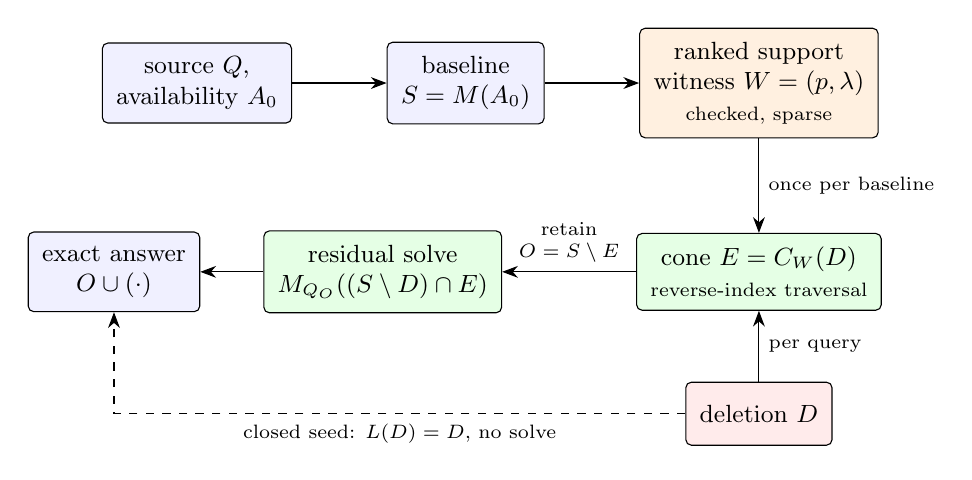
\begin{tikzpicture}[>={Stealth[length=2mm]},font=\small,
  box/.style={draw,rounded corners=2pt,minimum height=8mm,inner sep=5pt,align=center},
  region/.style={draw,rounded corners=4pt,inner sep=6pt}]
\node[box,fill=blue!6] (src) {source $Q$,\\ availability $A_0$};
\node[box,fill=blue!6,right=12mm of src] (base) {baseline\\ $S=M(A_0)$};
\node[box,fill=orange!12,right=12mm of base] (wit) {ranked support\\ witness $W=(p,\lambda)$\\ \scriptsize checked, sparse};
\node[box,fill=green!10,below=12mm of wit] (cone) {cone $E=C_W(D)$\\ \scriptsize reverse-index traversal};
\node[box,fill=green!10,left=17mm of cone] (res) {residual solve\\ $M_{Q_O}((S\setminus D)\cap E)$};
\node[box,fill=blue!6,left=8mm of res] (ans) {exact answer\\ $O\cup(\cdot)$};
\node[box,fill=red!8,below=9mm of cone] (del) {deletion $D$};
\draw[->] (src) -- (base);
\draw[->] (base) -- (wit);
\draw[->] (wit) -- node[right,font=\scriptsize]{once per baseline} (cone);
\draw[->] (del) -- node[right,font=\scriptsize]{per query} (cone);
\draw[->] (cone) -- node[above,font=\scriptsize,align=center]{retain\\ $O=S\setminus E$} (res);
\draw[->] (res) -- (ans);
\draw[->,dashed] (del.west) -| node[below,font=\scriptsize,pos=0.25]{closed seed: $L(D)=D$, no solve} (ans.south);
\end{tikzpicture}
\caption{Certified localization of one deletion query. The witness is computed once from the source and checked; a query traverses the selected graph from the deleted reactions, retains the complement of the cone without any recomputation, and resolves the cone by one residual maximum-RAF computation with the retained products adjoined to the food. If no selected edge leaves $D$, the loss is $D$ itself.}
\label{fig:pipeline}
\end{figure}

\begin{proposition}[closed-seed shortcut]\label{prop:closedseed}
Let $W$ be valid on $S$ and $K\subseteq S$. If $t\in K$ whenever $t\in S$, $r\in K$ and $r\in p(t)$ (no selected edge leaves $K$), then $L(K)=K$.
\end{proposition}

\begin{proof}
The hypothesis gives $C_W(K)\subseteq K$, so $L(K)\subseteq K$ by Theorem~\ref{thm:localization}; extensivity gives the converse.
\end{proof}

\subsection{Checking the residual computation}\label{sec:checking}

The implementation stores the baseline as a mask together with, for each molecule, the number of baseline reactions producing it. For a molecule needed as a reactant or catalyst inside the region, subtracting the producers that lie in $E$ leaves a count; a positive remainder certifies supply by $O$. These molecules, with food, form the residual boundary; products of $O$ that no local reaction needs may be omitted, since induction on local closure preserves every reactant and catalyst test.

The residual maximum RAF is itself certified. A \emph{closure certificate} is a finite reaction schedule: replay starts from food and adds the products of a scheduled reaction only when it is available and its reactants are present, so the replayed pool is always contained in the true closure; the checker then verifies that the pool is closed under every available reaction, and leastness gives the reverse inclusion. A \emph{pruning certificate} supplies such schedules for the successive decreasing reaction sets and is accepted only on a round that is a fixed point. Induction over accepted rounds shows that the returned set is the residual maximum; on rejection the implementation falls back to a literal fresh evaluation, so a malformed proposal cannot change an answer. Theorem~\ref{thm:localization} then proves exactness of every accepted localized answer. The sequential engine additionally supports insertions under stronger source-derived dependency conditions and commits no state before certificate acceptance.

\subsection{A charge-model amortization theorem}\label{sec:family}

We now state the one result of this paper that concerns cost rather than correctness. It is a theorem in a declared charge model, not a native runtime claim.

Consider the family with $n$ pairs and $m=2n+1$ reactions: food $\{f\}$, a hub reaction $f\to h$ catalysed by $f$, and for each $i$ the reactions $h\to a_i$ catalysed by $b_i$ and $h\to b_i$ catalysed by $a_i$, all species distinct. Every reaction is incident with $h$, so the reaction--molecule incidence graph is connected, and every stoichiometric column has a unique positive product coordinate, so no two columns are positive scalar multiples of one another. Each pair is a catalytic two-cycle: neither reaction has its catalyst before the other fires, which is exactly the situation that ordinary RAF semantics admits and that condition (W2) accommodates.

An \emph{edit packet} is five words: a pair index, two removal bits and two addition bits, removal applied before addition. The packet generates its two-reaction region, a two-round pruning certificate whose schedules are $[\text{left},\text{right}]$ and $[\,]$, and the right reaction as a membership target. The \emph{charge semantics} prices identifier comparisons, cached reads, Boolean branches, bounded-word arithmetic, finite-set comparisons and copies, certificate replay, state changes and output construction; all tariffs are executable definitions in the Lean development. The \emph{fresh point baseline} scans its $m$-entry availability representation on every query, so its charge is at least $mq$ on $q$ queries.

\begin{theorem}[charge-model amortization]\label{thm:family}
Let $m=2n+1$ and let $P(n)$ be the explicit setup cap below. For every positive integer $t$ with $1150\,t\le m$, every initial availability $A$ and every valid pair-edit sequence of length $q>P(n)$, the arithmetic packet evaluator returns the literal sequential maximum-RAF membership trace and
\[
t\cdot\mathrm{charge}(\text{packet evaluator})<\mathrm{charge}(\text{fresh point baseline}).
\]
The conclusion also records hub incidence and the distinct-positive-ray property of the family. With $p=m+1$,
\begin{align*}
T(e,i,o,p)&=1+e(i+1)(p+1)+2(p+eo+1)^{2},\\
H(e,i,c,p)&=1+e(i+c+2)(p+1)+2(e+1)^{2},\\
R(e,i,o,c,p)&=p+p\,T(e,i,o,p)+H(e,i,c,p),\\
P(n)&=m(14m+13+2p)+\big(m+m\,R(m,1,1,1,p)\big)\\
&\qquad+\big(2m+p+m+2m(m+1)+p(m+1)^{2}\big).
\end{align*}
\end{theorem}

\begin{proof}[Proof sketch]
Source compilation constructs dependency and needs vectors once, computes the initial maximum, and builds masks and producer counts; its charge is bounded by $P(n)$ by direct substitution of the executable tariffs. A pair region contains two reactions with needed-row total $4$ and product-row total $2$; substitution into the charged local bounds gives region checking at most $19$, boundary charge $155$ and total local certificate charge at most $818$, hence a local cap of $831$ with metadata, an accepted-transaction budget of $1011$ after edit preparation and state update, a cached per-query charge of $1014$ after dispatch, target lookup and output construction, and at most $135$ more for five-word decoding, arithmetic reaction codes and generated cells. The total is at most $P(n)+1149q<1150q$ when $q>P(n)$. Multiplying by $t$ and using $1150t\le m\le$ (baseline charge per query) proves the inequality. Packet refinement proves that both evaluators return the same literal trace. The formal statement is \lean{RAFQueryCompilation.ModuleFamily.family\_terminal\_factor}.
\end{proof}

Factors are unbounded: take $n=575t$ and any sufficiently long valid edit list. The cap $P(n)$ is conservative, so the sufficient $q$ can be enormous; the theorem establishes a structural amortization factor, not a numerical prediction of native break-even. It is a comparison with a specified fresh algorithm, not an information-theoretic lower bound on all RAF algorithms or on a family-specialized answer table.

\subsection{Implementation measurements}\label{sec:localization-impl}

The measured implementation is the ranked-witness deletion-loss route of Theorem~\ref{thm:localization} with the certificate bridge of Section~\ref{sec:checking}, not the packet interpreter of Theorem~\ref{thm:family}. Two synthetic balanced source generators were used. In the \emph{two-step} family a hub $f\to x$ feeds reactions $U_i:f+x\to b_i+c_i$ and $V_i:f+b_i\to x+a_i$, with $V_i$ food-catalysed and $U_i$ catalysed by the preceding $a$ in a fixed group; in the \emph{reexport} family reactions $f+x\to x+a_i$ use preceding group products as catalysts. Both have distinct nonproportional columns and connected incidence graphs; neither is biological data. For each source the complete singleton-deletion profile, one loss list per baseline reaction, was computed and compared entry by entry with two independently implemented Python references, active-producer closure/pruning and pseudo-RAF pruning after \citep{hordijk2015}; these are not the authors' native implementation.

\begin{table}[t]
\centering\small
\begin{tabular}{@{}p{0.44\linewidth}rrrr@{}}
\toprule
Profile & Queries & Witness (s) & Reference (s) & Ratio \\
\midrule
Two-step, 512 and 1024 pairs; producer plus checker & 3074 & 0.99 / 1.79 & --- & 5.10 / 7.61 \\
\quad same runs; complete cold session & 3074 & 25.96 & 18.67 & 0.72 \\
Two-step, 2048 pairs (4097 reactions); pipeline & 4097 & 5.11 & 58.18 & 11.38 \\
Reexport, 4096 peripheral (4097 reactions); pipeline & 4097 & 4.21 & 61.16 & 14.54 \\
\quad both sources; end to end with one cold launch & 8194 & 35.37 & 119.35 & 3.37 \\
\bottomrule
\end{tabular}
\caption{Single-run wall-clock observations on one Windows machine. All $3074+8194$ loss lists matched both references exactly. The second row shows why warm-only measurements are insufficient: a cold checker launch dominates a moderate workload. Timings are single observations, not confidence intervals.}
\label{tab:qc}
\end{table}

Table~\ref{tab:qc} reports the observations. Every deployed producer permits cone regions up to $64$ reactions before falling back to global closure; the threshold is a heuristic, and every proposed certificate is still checked. The gains are a scoped crossing on two synthetic families with one baseline pair; independent reproduction, heterogeneous perturbations and comparison with pinned native author implementations are not claimed.

\section{Witness selection}\label{sec:selection}

Theorem~\ref{thm:localization} holds for every valid witness, and different legal producer choices can produce very different cones. This section asks which witness to store for a workload of independent deletion queries against a fixed baseline. Neither sparsity nor chemical redundancy alone identifies a good choice.

\subsection{The objective and the intrinsic floor}

For nonnegative singleton weights $w:S\to\R_{\ge0}$, transposing the finite reachability relation gives
\begin{equation}\label{eq:objective}
J_w(W)=\sum_{d\in S}w_d\,|C_W(\{d\})|=\sum_{r\in S}\ \sum_{d\in\Anc_W(r)}w_d .
\end{equation}
Weights summing to one make this an expectation; all weights one give the total singleton cost, whose division by $n$ is the uniform mean. The objective is transitive reachability, not immediate out-degree or parent count. We also consider the worst singleton cone $\max_{d}|C_W(\{d\})|$ and, in Section~\ref{sec:selection-impl}, complete implementation cost; these objectives can prefer different witnesses, and reducing the mean can increase the maximum.

\begin{proposition}[intrinsic floor]\label{prop:floor}
For any finite deletion workload with probabilities $\mu(K)$ and any valid $W$,
\[
\E_\mu|C_W(K)|=\E_\mu|L(K)|+\E_\mu|C_W(K)\setminus L(K)|.
\]
\end{proposition}

\begin{proof}
Theorem~\ref{thm:localization} gives $L(K)\subseteq C_W(K)$; partition and take weighted sums. The Lean statement \lean{expected\_cone\_decomposition} holds for any finite real weighting.
\end{proof}

Selecting $W$ therefore changes only the excess above a structural floor that no witness can lower.

\subsection{Perfect queries, intrinsic dependence and synergy}

\begin{theorem}[perfect individual queries]\label{thm:perfect}
For every $K\subseteq S$ there is a valid witness $W_K$ with $C_{W_K}(K)=L(K)$. Equivalently,
\[
L(K)=\bigcap_{W\text{ valid on }S}C_W(K).
\]
\end{theorem}

\begin{proof}
Put $T=M(S\setminus K)$, a fixed set with $T\cap K=\emptyset$. By Lemma~\ref{lem:existence}, $T$ has a witness with parents inside $T$; keep its ranks and parents on $T$. Choose a food-generation ordering of $S$ and assign each $r\in S\setminus T$ a rank above the maximum rank on $T$, increasing along the ordering. For such $r$ and a nonfood reactant $x$, the ordering supplies an earlier producer $t\in S$ of $x$: if $t\in T$ its rank is smaller because all ranks on $T$ are; if $t\in S\setminus T$ it is earlier in the ordering. Select it. Select any catalytic witness of $r$ in $S$. No selected edge enters $T$ from $S\setminus T$ because parents of reactions of $T$ were chosen in $T$. The cone of $K$ starts in $S\setminus T$ and cannot enter $T$, so $C_{W_K}(K)\subseteq S\setminus T=L(K)$; Theorem~\ref{thm:localization} gives equality. The intersection formula follows since every valid cone contains $L(K)$.
\end{proof}

The construction is an existence argument: it computes $T$ first, so it does not accelerate that first query. It does say that the true loss is exactly what all witnesses agree on.

\begin{theorem}[intrinsic singleton dependence]\label{thm:preorder}
On $S$ define $d\preccurlyeq r$ when $r\in L(\{d\})$. This relation is reflexive and transitive; mutual dependence is an equivalence relation.
\end{theorem}

\begin{proof}
Reflexivity is extensivity of $L$. For transitivity, by Theorem~\ref{thm:perfect}, $d\preccurlyeq r$ means that $r\in C_W(\{d\})$ for every valid $W$. If $a\preccurlyeq b$ and $b\preccurlyeq c$ then in each fixed valid selected graph there is a path from $a$ to $b$ and one from $b$ to $c$, hence one from $a$ to $c$; applying the intersection formula again yields $a\preccurlyeq c$. (Alternatively, use the last clause of Proposition~\ref{prop:lossclosure}.)
\end{proof}

The equivalence classes consist of reactions mutually indispensable for one another's survival within the fixed baseline. A class need not itself be a RAF. Dependence is intrinsic even though any one selected graph may contain additional paths.

\begin{theorem}[synergy forces singleton overestimation]\label{thm:synergy}
If a valid witness $W$ is perfect for every singleton, $C_W(\{d\})=L(\{d\})$ for all $d\in S$, then it is perfect for every deletion set. Consequently, defining the \emph{synergy}
\[
\Delta(K)=L(K)\setminus\bigcup_{d\in K}L(\{d\}),
\]
if $\Delta(K)\neq\emptyset$ for some $K\subseteq S$ then no single valid witness is perfect for every singleton.
\end{theorem}

\begin{proof}
A path from a seed set starts at one of its elements, so $C_W(K)=\bigcup_{d\in K}C_W(\{d\})$. Under singleton perfection this equals $\bigcup_{d\in K}L(\{d\})\subseteq L(K)$ by monotonicity, while $L(K)\subseteq C_W(K)$ by Theorem~\ref{thm:localization}. Hence equality holds throughout and $\Delta(K)=\emptyset$. The second claim is the contrapositive. No converse is claimed.
\end{proof}

\begin{example}[two interchangeable producers]\label{ex:twoproducer}
Let two food-consuming, food-catalysed producers $P_0,P_1$ both produce $x$, and let $m$ food-catalysed consumers $e_1,\dots,e_m$ consume $x$. Every actual singleton loss has size one. A normalized witness assigns $k$ consumers to $P_0$ and $m-k$ to $P_1$; the producer cones have sizes $1+k$ and $1+m-k$ and each consumer cone has size one. Since normalization removes parents without enlarging cones,
\[
\min_{W}\max_{d\in S}|C_W(\{d\})|=1+\lceil m/2\rceil .
\]
The best uniform mean is $(2m+2)/(m+2)\to2$ against an intrinsic floor of $1$, whereas the producer-weighted mean is $1+m/2$. Deleting both producers loses every consumer although each producer deletion alone loses nothing else, so $\Delta(\{P_0,P_1\})\neq\emptyset$ and Theorem~\ref{thm:synergy} applies. The example proves an unbounded worst-case or producer-weighted gap, not an unbounded uniform-mean gap.
\end{example}

\subsection{An exactly solvable class and the downstream-convergence wall}

\begin{theorem}[one-layer weighted optimality]\label{thm:onelayer}
Let $P$ be a finite producer set and $U$ a finite consumer set, with a nonempty allowed set $A_i\subseteq P$ for each $i\in U$. Construct the reactions
\[
p_j:\ f\to u_j+\{x_i:j\in A_i\},\qquad e_i:\ x_i\to y_i,
\]
where $f$ is food, all other displayed molecules are distinct, and $f$ catalyses every reaction. The full reaction set is a RAF. For nonnegative singleton weights $w$, choosing for each $e_i$ a producer of minimum weight $w_{p_j}$ among $j\in A_i$ yields a witness that is globally optimal for $J_w$ over all valid witnesses, of any parents and ranks.
\end{theorem}

\begin{proof}
Any valid witness includes among the parents of $e_i$ an allowed producer of $x_i$. Retain one such parent per consumer and delete all other parents: this is valid with producers at rank $0$ and consumers at rank $1$, and deleting parents cannot increase reachability. For a normalized choice $a(i)\in A_i$ the ancestors of a producer are itself and the ancestors of $e_i$ are $\{e_i,p_{a(i)}\}$, so by \eqref{eq:objective}
\[
J_w(a)=\sum_{r\in P\cup U}w_r+\sum_{i\in U}w_{p_{a(i)}} .
\]
The second sum separates over $i$, and a least-weight allowed producer minimizes each term. Normalization gives optimality against arbitrary witnesses, not only normalized ones.
\end{proof}

For uniform weights the one-layer total is $|P|+2|U|$ regardless of assignment. One additional reaction destroys this independence.

\begin{theorem}[exact set-cover equivalence]\label{thm:setcover}
Augment the source of Theorem~\ref{thm:onelayer} by one reaction $t$ requiring every $y_i$, producing a fresh molecule $z$, and catalysed by $f$; let $m=|P|$ and $n=|U|$. There is a valid witness with total uniform singleton cost at most $m+3n+1+q$ if and only if the incidence system $(A_i)_{i\in U}$ has a cover $B\subseteq P$ with $|B|\le q$ and $A_i\cap B\neq\emptyset$ for every $i$.
\end{theorem}

\begin{proof}
Each $y_i$ has the unique producer $e_i$, so every $e_i$ is a forced parent of $t$ in every witness. Normalize the remaining parents as before; the ranks are $0,1,2$. The ancestor counts are $1$ for each producer, $2$ for each $e_i$, and $1+n+|\im a|$ for $t$, so $J_1(a)=m+3n+1+|\im a|$. The image of $a$ is a cover; conversely a cover $B$ supplies a choice $a(i)\in A_i\cap B$ with $|\im a|\le|B|$. Normalization never increases cost, which gives both directions. Nonempty $A_i$ make the whole constructed source its own maximum RAF. The aggregator makes shared producer ancestry observable and couples the previously independent choices.
\end{proof}

\begin{theorem}[NP-completeness of mean selection]\label{thm:npc}
The problem: given a finite catalytic reaction system in explicit incidence encoding, a baseline maximum RAF $S$, and a rational threshold $\theta$ in binary, decide whether some ranked support witness on $S$ has uniform mean singleton cone size at most $\theta$; is NP-complete. Hardness already holds for the food-catalysed three-level sources of Theorem~\ref{thm:setcover}.
\end{theorem}

\begin{proof}
\emph{Membership.} A witness is encoded by a parent adjacency matrix restricted to $S$ (parents outside $S$ are irrelevant) and one rank per reaction; replacing ranks by their position among the distinct ranks on $S$ preserves all strict comparisons and bounds ranks by $|S|-1$, so the certificate has $O(|S|^{2}+|S|\log|S|)$ bits. Validity is checked by scanning reactant, product, parent and catalyst incidences. Reachability from each baseline reaction is computed in $O(|S|^{3})$ time; the total cone size is an integer at most $|S|^{2}$, and comparing its ratio to $|S|$ with $\theta$ is polynomial-bit integer arithmetic. If the baseline is supplied as $M(A_0)$ it is computed first by closure and pruning in polynomial time.

\emph{Hardness.} Reduce from set cover \citep{karp1972} with $m$ sets, $n$ elements and $\ell$ incidences. Theorem~\ref{thm:setcover} constructs $m+n+1$ reactions, $m+2n+2$ molecules and $O(m+n+\ell)$ incidences, with threshold $\theta=(m+3n+1+q)/(m+n+1)$ of polynomial bit length. Instances with an uncovered element are recognized in polynomial time and mapped to a fixed no-instance, so all $A_i$ may be assumed nonempty and the full reaction set is the baseline. Theorem~\ref{thm:setcover} is the yes/no equivalence.
\end{proof}

The additive term $m+3n+1$ matters: a multiplicative approximation to the total singleton cost does not translate into the same multiplicative approximation to $|\im a|$ after subtracting it, so no set-cover approximation threshold \citep{feige1998} is transferred. Nor does the reduction classify the worst-singleton objective. The finite source, normalization, baseline identity and threshold equivalence are compiled in Lean; the encoding argument is conventional.

\subsection{Portfolios: exact answers, greedy selection, and an exponential wall}

Let $H$ be a finite pool of valid witnesses and $\mathcal P\subseteq H$ a portfolio. For a deletion $K\subseteq S$ define
\[
O_{\mathcal P}(K)=\bigcup_{W\in\mathcal P}\big(S\setminus C_W(K)\big),\qquad D_{\mathcal P}(K)=S\setminus O_{\mathcal P}(K).
\]
For a nonempty portfolio $D_{\mathcal P}(K)=\bigcap_{W\in\mathcal P}C_W(K)$; for the empty portfolio $D_\emptyset(K)=S$ and the method is a fresh solve.

\begin{theorem}[exact portfolio residual]\label{thm:portfolio}
For every nonempty portfolio $\mathcal P$ and every $K\subseteq S$, with $O=O_{\mathcal P}(K)$,
\[
M(S\setminus K)=O\cup M_{Q_O}\big((S\setminus K)\setminus O\big).
\]
\end{theorem}

\begin{proof}
Each $S\setminus C_W(K)$ is parent-closed for its own witness, hence a fixed set by Theorem~\ref{thm:retention}, and it avoids $K$. A union of fixed sets is a fixed set, since the supporting closures of each member are contained in the closure of the union. Apply Theorem~\ref{thm:residual} with $A=S\setminus K$ and $I=(S\setminus K)\setminus O$.
\end{proof}

The answer is exact even when $D_{\mathcal P}(K)$ strictly contains $L(K)$, and the intersection need not be a cone of any one witness; soundness comes from the retained union.

For a finite training set $\mathcal T$ of deletion queries, the \emph{rescue events} of $W$ are the pairs $(K,r)$ with $K\in\mathcal T$ and $r\in S\setminus C_W(K)$, and $G(\mathcal P)$ counts the events covered by at least one member of $\mathcal P$.

\begin{theorem}[greedy portfolio selection]\label{thm:greedy}
For nonempty $H$ and $b\ge1$, repeatedly add a member of $H$ with maximum new rescue count. After $b$ steps the portfolio $\mathcal P_b$ has at most $b$ members, yields the exact answer of Theorem~\ref{thm:portfolio} for every deletion query, and
\[
G(\mathcal P_b)\;\ge\;\Big[1-\big(1-\tfrac1b\big)^{b}\Big]\max_{\mathcal B\subseteq H,\ |\mathcal B|\le b}G(\mathcal B).
\]
\end{theorem}

\begin{proof}
Coverage is monotone with diminishing marginal gains. For a comparison portfolio $\mathcal B$ of size at most $b$, at step $j$ the gap $G(\mathcal B)-G(\mathcal P_j)$ is at most the sum of the marginal gains of the members of $\mathcal B$, hence at most $b$ times the largest available gain; greedy reduces the gap by at least a $1/b$ fraction, and iterating from zero gives the bound \citep{nemhauser1978}. Every selected candidate belongs to $H$ and is valid, so Theorem~\ref{thm:portfolio} applies regardless of the workload.
\end{proof}

The guarantee concerns rescued training mass relative to the best same-budget portfolio in the supplied pool; it is not a residual-cost, runtime, all-witness, or unseen-query guarantee. Exactness of unseen answers is unconditional.

\begin{theorem}[sharp portfolio size]\label{thm:exponential}
For each integer $k\ge0$ there is a food-catalysed source with $2k+1$ reactions whose maximum RAF is the full set and on which the minimum number of witnesses whose cone intersection equals $L(K)$ for every deletion set $K$ is exactly $2^{k}$. For $k\ge1$, two complementary witnesses achieve exact intersections for every singleton deletion, and one does not.
\end{theorem}

\begin{figure}[t]
\centering
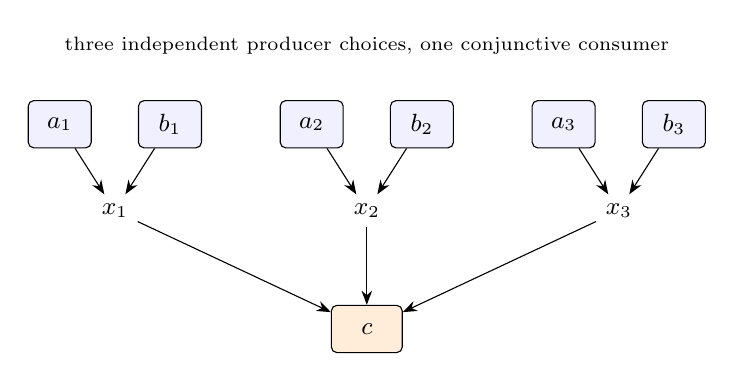
\begin{tikzpicture}[>={Stealth[length=1.8mm]},font=\small,
  prod/.style={draw,rounded corners=2pt,minimum width=8mm,minimum height=6mm,fill=blue!6},
  cons/.style={draw,rounded corners=2pt,minimum width=9mm,minimum height=6mm,fill=orange!15}]
\foreach \i/\x in {1/0,2/3.2,3/6.4}{
  \node[prod] (a\i) at (\x-0.7,2) {$a_{\i}$};
  \node[prod] (b\i) at (\x+0.7,2) {$b_{\i}$};
  \node (x\i) at (\x,0.9) {$x_{\i}$};
  \draw[->] (a\i) -- (x\i);
  \draw[->] (b\i) -- (x\i);
}
\node[cons] (c) at (3.2,-0.6) {$c$};
\draw[->] (x1) -- (c);
\draw[->] (x2) -- (c);
\draw[->] (x3) -- (c);
\node[font=\scriptsize,align=center] at (3.2,3) {three independent producer choices, one conjunctive consumer};
\end{tikzpicture}
\caption{The paired source for $k=3$. Each producer consumes food and produces its own private molecule together with the shared $x_i$; food, catalyst and private-product incidences are suppressed. The consumer $c$ requires all $x_i$. A witness must choose one parent per pair for $c$, and each choice is defeated by the deletion of exactly the chosen producers.}
\label{fig:paired}
\end{figure}

\begin{proof}
Construct producer pairs $a_i,b_i$ for $i=1,\dots,k$, each consuming food $f$ and producing $x_i$ together with a private product, and one reaction $c$ consuming all $x_i$ and producing a fresh product; every reaction is catalysed by $f$ (Figure~\ref{fig:paired}). Producers have rank $0$ and $c$ rank $1$; the full set is a RAF.

\emph{Lower bound.} A valid witness must contain in $p(c)$ at least one of $a_i,b_i$ for each $i$, because nothing else produces $x_i$; choosing one per pair extracts an assignment $\alpha\in\{0,1\}^{k}$ from every witness, whatever its extra parents or ranks. For $\beta\in\{0,1\}^{k}$ let $K_\beta$ delete the producer of each pair \emph{not} chosen by $\beta$. Every undeleted producer survives and supplies its pair's input, so $c$ survives and $L(K_\beta)=K_\beta$. If $\alpha\ne\beta$, some selected parent of $c$ lies in $K_\beta$ and $c\in C_W(K_\beta)$. A fixed witness therefore excludes $c$ for at most one of the $2^{k}$ queries; a portfolio with fewer members misses some $\beta$, and its intersection contains $c$ although the loss does not.

\emph{Attainability.} Store every normalized assignment witness $W_\alpha$. Its cone of $K$ contains $K$ and contains $c$ exactly when $c\in K$ or a selected producer lies in $K$. If $c$ is neither deleted nor deprived of some pair entirely, choose an undeleted producer per pair; that witness's cone excludes $c$. Otherwise $c$ is actually lost and lies in every cone. Producers have no parents, so their cone membership is exactly membership in $K$. Hence the intersection over the full pool is $L(K)$ for every $K$.

\emph{Singletons.} For a producer deletion one of the two constant assignments avoids it, so their cone intersection is exact; a singleton deletion of $c$ is exact in both. For $k\ge1$ any single witness chooses a parent of $c$, and deleting that parent alone leaves its mate and $c$ alive while the cone contains $c$. For $k=0$ one witness suffices, consistent with $2^{0}=1$.
\end{proof}

These are representation-size bounds for exact regions obtained by intersecting cones. By Theorem~\ref{thm:portfolio} a small portfolio still returns exact answers; the theorem shows that singleton tests can substantially understate the storage required for universal exact-region compilation. The Lean lower bound quantifies over arbitrary valid witness families indexed by any finite type of cardinality less than $2^{k}$; the consumer has arity $k$, and a bounded-arity refinement is not claimed.

\subsection{Implementation evidence and adoption rule}\label{sec:selection-impl}

The implementation treats proposed witnesses as untrusted. A canonical one-layer constructor implements Theorem~\ref{thm:onelayer}; for general sources a bounded proposer enumerates source-allowed witness slots, separates reactant rank inequalities from catalytic choices, rejects reactant cycles and scores actual reachability, with a default assignment limit of $4096$ beyond which a validated default is returned labelled feasible rather than optimal.

A held-out study used sixteen distinct $48$-reaction sources, four independent seeds in each of four synthetic mechanisms, with every distinct singleton deletion, $768$ queries per strategy. All loss outputs agreed with the two independent references. Table~\ref{tab:portfolio} reports complete session medians. Portfolios of three and five charge two and four survivor-construction solves respectively, together with memory, cone discovery, boundary work and outputs. A separate five-seed $128$-reaction overlap profile gave a median single-witness session of $2.756$\,ms against $55.157$\,ms for active fresh evaluation, while a seed-first three-witness portfolio took $10.470$\,ms even though $127$ of $128$ queries per source qualified for the closed-seed shortcut: portfolio setup and repeated discovery consumed the region savings.

\begin{table}[t]
\centering\small
\begin{tabular}{@{}lrrrr@{}}
\toprule
Source mechanism & One witness & Portfolio 3 & Portfolio 5 & Active fresh \\
\midrule
Overlapping inputs & 1.013 & 2.881 & 3.978 & 7.690 \\
Catalytic feedback & 3.478 & 7.842 & 14.147 & 15.261 \\
Redundant reexport & 0.918 & 3.522 & 5.724 & 5.803 \\
Mixed depth & 5.388 & 7.624 & 11.450 & 7.686 \\
\bottomrule
\end{tabular}
\caption{Median complete Python session times in milliseconds over four distinct $48$-reaction source instances per row; witness strategies include the closed-seed test. Descriptive medians, not confidence intervals or native timings.}
\label{tab:portfolio}
\end{table}

Applying the mean-optimizing selector to the $32$ held-out sources of Section~\ref{sec:robustness} plus a cooperative fixture, all $196$ deletion queries per strategy returned identical exact loss sets; the sum of cone sizes fell from $499$ to $480$ while measured setup rose from $1.80$ to $4.09$\,ms and query time changed from $2.68$ to $2.72$\,ms. On an eight-reaction aggregator the native checker accepted $22$ singleton queries under default and mean-optimal witnesses with zero mismatches; total singleton cones fell from $17$ to $15$ while the worst cone rose from $3$ to $5$.

For a homogeneous workload of $Q$ queries, an extra setup cost $H$ is repaid only when $H+Q\,t_{\mathrm{reuse}}<Q\,t_{\mathrm{fresh}}$, with per-query terms including discovery, residual evaluation and output. This is accounting, not a theorem. The measured decision is to prefer one checked witness with the closed-seed shortcut in the tested Python profiles, and fresh evaluation for a short cold native workload; larger portfolios are justified only by a declared coverage objective or complete measured savings.

\section{Exact robustness laws under random deletion}\label{sec:robustness}

We now leave algorithms and ask which features of the source determine damage. Let $A_p\subseteq S$ retain each reaction of the baseline independently with probability $p$, and define
\[
\Phi(p)=\E|M(A_p)|,\qquad F(p)=\Pr[M(A_p)\neq\emptyset].
\]
Both are polynomials in $p$, defined for all real $p$ though probabilities refer to $0\le p\le1$. All probability statements use independent availability in one fixed source; catalytic relations are never resampled, and no finite robustness curve establishes a thermodynamic singularity.

\subsection{First and second order at the all-retained endpoint}

For a real observable $H$ on subsets of $S$ and a coordinate $i$, write $A_p^{-i}$ for independent availability on $S\setminus\{i\}$. Grouping the product-measure expectation by one coordinate, differentiating its affine dependence on that coordinate, and then moving all coordinates together gives the Russo--Margulis formula \citep{margulis1974,russo1981,odonnell2014}
\begin{equation}\label{eq:russo}
\frac{d}{dp}\,\E H(A_p)=\sum_{i\in S}\E\big[H(A_p^{-i}\cup\{i\})-H(A_p^{-i})\big].
\end{equation}

\begin{proposition}[first-order sensitivity]\label{prop:firstorder}
\[
\Phi'(1)=\sum_{i\in S}|L(\{i\})|,\qquad F'(1)=\big|\{i\in S: M(S\setminus\{i\})=\emptyset\}\big| .
\]
\end{proposition}

\begin{proof}
At $p=1$ the summand of \eqref{eq:russo} is $H(S)-H(S\setminus\{i\})$. For size this is $n-|M(S\setminus\{i\})|=|L(\{i\})|$; for the nonempty indicator, monotonicity makes it the indicator of the pivotal event $M(S\setminus\{i\})=\emptyset$. No division by $p(1-p)$ is involved.
\end{proof}

\begin{theorem}[curvature balances overlap and cooperation]\label{thm:curvature}
For distinct $i,j\in S$ put $C_{ij}=L(\{i,j\})\setminus\big(L(\{i\})\cup L(\{j\})\big)$. Then, summing once over each unordered pair,
\[
\Phi''(1)=2\sum_{\{i,j\}\subseteq S}\Big(|L(\{i\})\cap L(\{j\})|-|C_{ij}|\Big).
\]
\end{theorem}

\begin{proof}
Differentiate \eqref{eq:russo} once more. Each coordinate difference is independent of its own coordinate, so the second sum runs over ordered pairs of distinct coordinates, and at $p=1$ the pair $(i,j)$ contributes
\[
|S|-|M(S\setminus\{i\})|-|M(S\setminus\{j\})|+|M(S\setminus\{i,j\})|=|L(\{i\})|+|L(\{j\})|-|L(\{i,j\})| .
\]
Monotonicity gives $L(\{i\})\cup L(\{j\})\subseteq L(\{i,j\})$; split $L(\{i,j\})$ into that union and its complement $C_{ij}$, and apply inclusion--exclusion. The summand is symmetric, and ordered pairs count it twice.
\end{proof}

\begin{corollary}[small-deletion expansion]\label{cor:taylor}
Delete each reaction independently with probability $q=1-p$ and let $D_q$ be the deleted set. Then
\[
\E|L(D_q)|=q\sum_{i}|L(\{i\})|+q^{2}\sum_{\{i,j\}}\Big(|C_{ij}|-|L(\{i\})\cap L(\{j\})|\Big)+O(q^{3}).
\]
\end{corollary}

\begin{proof}
The left side is $n-\Phi(1-q)$ with $\Phi(1)=n$; expand the polynomial $\Phi$ at $1$ and use Proposition~\ref{prop:firstorder} and Theorem~\ref{thm:curvature}. The remainder is for each fixed finite source and is not uniform in the source size.
\end{proof}

Overlap makes repeated deletions partly redundant; cooperative failure makes a pair's joint effect exceed the singleton prediction. There is no universal sign. A catalytic cycle of length $\ell\ge2$ has $\Phi(p)=\ell p^{\ell}$ and $\Phi''(1)=\ell^{2}(\ell-1)>0$. Two food-catalysed producers of a common molecule and one food-catalysed consumer requiring it give $\Phi(p)=2p+2p^{2}-p^{3}$ and $\Phi''(1)=-2$: the only cooperative pair is the two producers, each of which spares the consumer alone.

\subsection{One-site catalyst choice and forward exposures}

\begin{lemma}[one-site decomposition]\label{lem:onesite}
Let $C_0,C_1$ be two catalyst maps on the same reaction system that agree at every reaction other than $v$, and let $C_\vee=C_0\cup C_1$ pointwise. Then for every availability set $A$,
\[
M_\vee(A)=M_0(A)\cup M_1(A).
\]
\end{lemma}

\begin{proof}
Every RAF for $C_0$ or $C_1$ is a RAF for $C_\vee$, giving one inclusion. Let $T$ be a RAF under $C_\vee$. If $v\notin T$ the three maps agree on $T$. If $v\in T$, choose a catalyst of $v$ in $\cl_T(F)$; it belongs to $C_0(v)$ or $C_1(v)$, and in that branch every other reaction of $T$ keeps its catalytic witness because the maps agree there, while food generation is unchanged. So $T$ is a RAF in one branch, and the union over RAF witnesses gives the other inclusion. The argument assumes nothing about reactants or products.
\end{proof}

We now specialize the source. A \emph{functional source} on a reaction set $R$ has every reaction $r$ consuming common food and producing its own private nonfood molecule $x_r$, no food catalysis, and $r$ catalysed by $x_{f(r)}$ for a map $f:R\to R$. At one distinguished reaction $v$ we allow instead either $x_{f(v)}$ or $x_{g(v)}$, where $g=f$ off $v$. The \emph{forward exposure} of $r$ under $f$ is the finite orbit
\[
O_f(r)=\{r,f(r),f^{2}(r),\dots\}.
\]

\begin{theorem}[all-deletion exposure law]\label{thm:exposure}
For every $A\subseteq R$, with $E_r=O_f(r)$ and $G_r=O_g(r)$,
\[
r\in M_\vee(A)\iff E_r\subseteq A\ \text{ or }\ G_r\subseteq A,
\qquad
\Pr[r\in M_\vee(A_p)]=p^{|E_r|}+p^{|G_r|}-p^{|E_r\cup G_r|}.
\]
\end{theorem}

\begin{proof}
In a functional source every RAF containing $r$ contains its unique catalyst producer $f(r)$, hence the whole orbit; conversely an available orbit is food-generated and supplies a catalyst for each of its members, so it is a RAF. Thus $r\in M_f(A)\iff O_f(r)\subseteq A$. Apply Lemma~\ref{lem:onesite}. The probability formula holds because retaining an orbit means retaining all its reactions, and retaining both means retaining their union; it preserves their shared randomness and is not a model of independent branch survival.
\end{proof}

The orbits are extracted from each \emph{resolved} source: an added catalyst can create a new self-sustaining cycle, and a witness computed before the addition can miss the rescue (Figure~\ref{fig:newcycle}).

\begin{figure}[t]
\centering
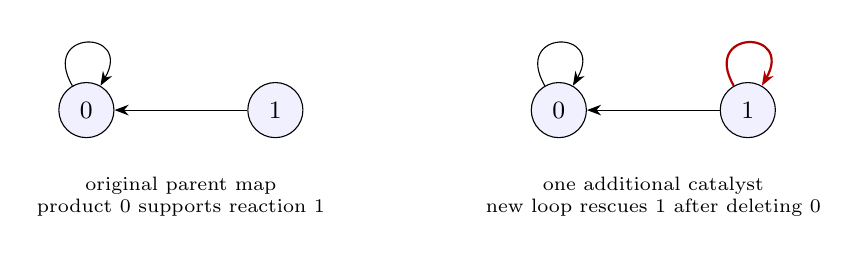
\begin{tikzpicture}[>={Stealth[length=1.8mm]},font=\small,
  rx/.style={draw,circle,minimum size=7mm,fill=blue!6}]
\begin{scope}
\node[rx] (a0) at (0,0) {$0$};
\node[rx] (a1) at (2.4,0) {$1$};
\draw[->] (a1) -- (a0);
\draw[->] (a0) to[out=120,in=60,looseness=6] (a0);
\node[font=\scriptsize,align=center] at (1.2,-1.1) {original parent map\\ product $0$ supports reaction $1$};
\end{scope}
\begin{scope}[xshift=6cm]
\node[rx] (b0) at (0,0) {$0$};
\node[rx] (b1) at (2.4,0) {$1$};
\draw[->] (b1) -- (b0);
\draw[->] (b0) to[out=120,in=60,looseness=6] (b0);
\draw[->,red!70!black,thick] (b1) to[out=120,in=60,looseness=6] (b1);
\node[font=\scriptsize,align=center] at (1.2,-1.1) {one additional catalyst\\ new loop rescues $1$ after deleting $0$};
\end{scope}
\end{tikzpicture}
\caption{A new witness must be extracted after a catalyst addition. Arrows point from a reaction to its required catalytic parent. Initially $f(0)=f(1)=0$. Adding the product of $1$ as a catalyst for $1$ supplies the second resolution $g(1)=1$; after deleting $0$, reaction $1$ survives through its new self-loop, which the old witness cannot see. All reactions consume food.}
\label{fig:newcycle}
\end{figure}

\subsection{Complete external cuts and one catalyst addition}

Fix a target $r$, write $E=E_r$, $G=G_r$, and exclude direct target deletion. Theorem~\ref{thm:exposure} gives
\[
r\notin M_\vee(R\setminus D)\iff D\cap E\neq\emptyset\ \text{ and }\ D\cap G\neq\emptyset .
\]

\begin{theorem}[all inclusion-minimal external cuts]\label{thm:cuts}
The inclusion-minimal sets $D$ with $r\notin D$ that lose $r$ are exactly
\[
\big\{\{x\}:x\in(E\cap G)\setminus\{r\}\big\}\ \cup\ \big\{\{x,y\}:x\in E\setminus G,\ y\in G\setminus E\big\}.
\]
\end{theorem}

\begin{proof}
Every cut meets both exposures. If it contains a shared element, that element alone is a cut and minimality forces the singleton. Otherwise choose one element in each exposure; neither is shared, their pair is a cut contained in the original, and minimality forces the pair. Conversely each displayed singleton meets both exposures and has no nonempty proper subset; each displayed pair meets both while each of its singletons misses one. The target itself lies in both exposures and is excluded.
\end{proof}

The minimum cardinality of an external cut is one if a shared external element exists, two if none exists and both exclusive parts are nonempty, and no external cut exists if either orbit is $\{r\}$. Inclusion-minimal pairs may coexist with singleton cuts (Figure~\ref{fig:venn}).

\begin{figure}[t]
\centering
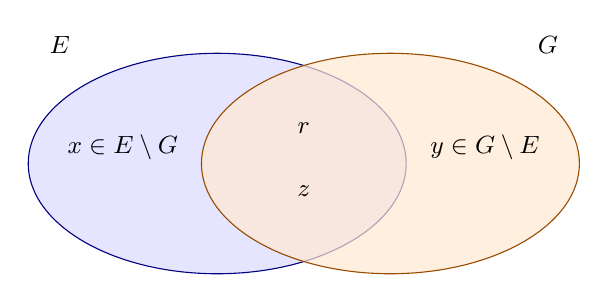
\begin{tikzpicture}[font=\small]
\draw[fill=blue!10,draw=blue!50!black] (0,0) ellipse (2.4 and 1.4);
\draw[fill=orange!18,draw=orange!60!black,fill opacity=0.7] (2.2,0) ellipse (2.4 and 1.4);
\node at (-1.2,0.2) {$x\in E\setminus G$};
\node at (3.4,0.2) {$y\in G\setminus E$};
\node at (1.1,0.45) {$r$};
\node at (1.1,-0.35) {$z$};
\node at (-2.0,1.5) {$E$};
\node at (4.2,1.5) {$G$};
\end{tikzpicture}
\caption{Shared and exclusive exposures have different meanings. A shared external element $z$ alone loses the target; a pair with one element from each exclusive region is inclusion-minimal even when a singleton cut exists. The target lies in the intersection but is excluded from external cuts.}
\label{fig:venn}
\end{figure}

\begin{theorem}[when a catalyst addition protects a target]\label{thm:gain}
Compare the functional source $f$ with the one-site union source. The exact target-survival gain is
\[
\Delta_r(p)=\Pr[r\in M_\vee(A_p)]-\Pr[r\in M_f(A_p)]=p^{|G_r|}\big(1-p^{|E_r\setminus G_r|}\big),
\]
which for $0<p<1$ is positive exactly when $E_r\setminus G_r\neq\emptyset$. The number of singleton deletions fatal to $r$ falls from $|E_r|$ to $|E_r\cap G_r|$, a reduction of $|E_r\setminus G_r|$.
\end{theorem}

\begin{proof}
Subtract $p^{|E_r|}$ from the formula of Theorem~\ref{thm:exposure} and use $|E_r\cup G_r|=|G_r|+|E_r\setminus G_r|$. The singleton count is Theorem~\ref{thm:cuts} with direct deletion included in both sources.
\end{proof}

Counting added catalysts alone does not identify protection: an added orbit contained in the old one gains nothing. For a supplied list of $c$ candidate single additions $(v,w)$, resolve each by $g(v)=w$ and $g=f$ elsewhere, sum $\Delta_r(p)$ over targets, and choose a maximizer; by linearity of expectation this maximizes expected surviving size over the list. Forward traversal constructs all orbits in $O(n^{2})$ parent visits per candidate, so the selector uses $O(cn^{2})$ expected elementary operations with hashed sets; precomputed powers reduce scoring to linear arithmetic once exposure sizes are known. No optimum for simultaneous multiple additions is claimed.

\subsection{Fluctuations and sufficient conditions for concentration}

\begin{theorem}[functional-source variance]\label{thm:variance}
In a functional source with $E_r=O_f(r)$ and $X=|M_f(A_p)|$,
\[
\Var(X)=\sum_{r,s\in R}\Big(p^{|E_r\cup E_s|}-p^{|E_r|+|E_s|}\Big).
\]
\end{theorem}

\begin{proof}
By Theorem~\ref{thm:exposure} in the one-parent case, $X=\sum_r I_r$ with $I_r$ the indicator of $E_r\subseteq A_p$. For each ordered pair $\E I_rI_s=p^{|E_r\cup E_s|}$ and $\E I_r\,\E I_s=p^{|E_r|+|E_s|}$; expand the variance of the finite sum. The identity includes the diagonal and holds at the endpoints.
\end{proof}

\begin{corollary}[sparse overlap suffices for concentration]\label{cor:concentration}
Let $K_n$ count the ordered pairs of reactions whose exposures intersect in an $n$-reaction source. For $0\le p\le1$,
\[
0\le\Var(X/n)\le K_n/n^{2}.
\]
If $K_n=o(n^{2})$ along a source sequence then $\Var(X/n)\to0$, so $X/n$ concentrates around its own expectation: for every $\varepsilon>0$, $\Pr[|X/n-\E X/n|>\varepsilon]\to0$. No limit for the expectations is assumed.
\end{corollary}

\begin{proof}
A disjoint pair has zero covariance because union cardinality is then the sum. Every other covariance is nonnegative, since the union has at most the sum of the cardinalities and $p\in[0,1]$, and is at most one. Sum and divide by $n^{2}$; Chebyshev's inequality gives the probability statement. The bounds also hold for varying retention probabilities provided the overlap condition holds.
\end{proof}

Orbit-size marginals do not determine the variance. The parent arrays $(0,2,0,4,0)$ and $(0,2,1,1,1)$ on five reactions both have sorted orbit sizes $(1,2,2,3,3)$ and sorted nonzero parent fan-outs $(1,1,3)$; at $p=1/2$ both means are $5/4$, but the variances are $9/4$ and $33/16$. Theorem~\ref{thm:variance} explains the difference exactly through the pairwise unions.

\subsection{Modules and gateways: two sharp controls}

\begin{proposition}[disjoint catalytic modules]\label{prop:modules}
Let the source be a nonempty finite family of disjoint private-product catalytic cycles of lengths $\ell_1,\dots,\ell_m$, possibly sharing food. Then, with $X=|M(A_p)|$,
\[
\Phi(p)=\sum_j\ell_jp^{\ell_j},\qquad F(p)=1-\prod_j\big(1-p^{\ell_j}\big),\qquad
\Var(X)=\sum_j\ell_j^{2}p^{\ell_j}(1-p^{\ell_j}),\qquad \Phi'(1)=\sum_j\ell_j^{2},
\]
Every singleton deletion destroys its entire module. If $N_k$ modules have length $k$ and $n=\sum_kkN_k$, a uniformly random singleton deletion has loss size $k$ with probability $kN_k/n$, and
\[
\Var(X/n)\le\frac{\sum_j\ell_j^{2}}{n^{2}}\le\frac{\ell_{\max}}{n}.
\]
\end{proposition}

\begin{proof}
A module survives exactly when all its reactions are present, and the module indicators are independent because their reaction sets are disjoint. The formulas follow; the size-bias statement counts reactions per module, and $\ell_j^{2}\le\ell_{\max}\ell_j$ gives the last bound.
\end{proof}

The size bias is a statement about counting, not about critical branching: module frequencies proportional to $k^{-5/2}$ on a finite range produce reaction-weighted loss frequencies proportional to $k^{-3/2}$ with no cascade between modules. A largest module of size $o(n)$ suffices for concentration without any assumption on the module-size distribution.

\begin{proposition}[common gateway]\label{prop:gateway}
Let every reaction, including reaction $0$ itself, be catalysed by the private product of reaction $0$, on $n$ reactions. Then $F(p)=p$ for every $n$, and conditional on retaining reaction $0$ the surviving size is $1+Y$ with $Y\sim\mathrm{Bin}(n-1,p)$ independent of that retention. Hence
\[
\Phi(p)=p+(n-1)p^{2},\qquad
\Var(X)=p(1-p)\big[1+(n-1)p\big]^{2}+(n-1)p^{2}(1-p),
\]
and for fixed $0<p<1$ the normalized variance $\Var(X/n)\to p^{3}(1-p)>0$.
\end{proposition}

\begin{proof}
Nonempty survival occurs exactly when reaction $0$ is retained, since every orbit passes through it and $\{0\}$ is a RAF. The conditional law and the law of total variance give the formulas.
\end{proof}

A persistent shared cause defeats concentration even though the availability coordinates are independent. This does not contradict Corollary~\ref{cor:concentration}: every pair of gateway exposures intersects, so $K_n=n^{2}$. Figure~\ref{fig:curves} plots the three exact curves.

\begin{figure}[t]
\centering
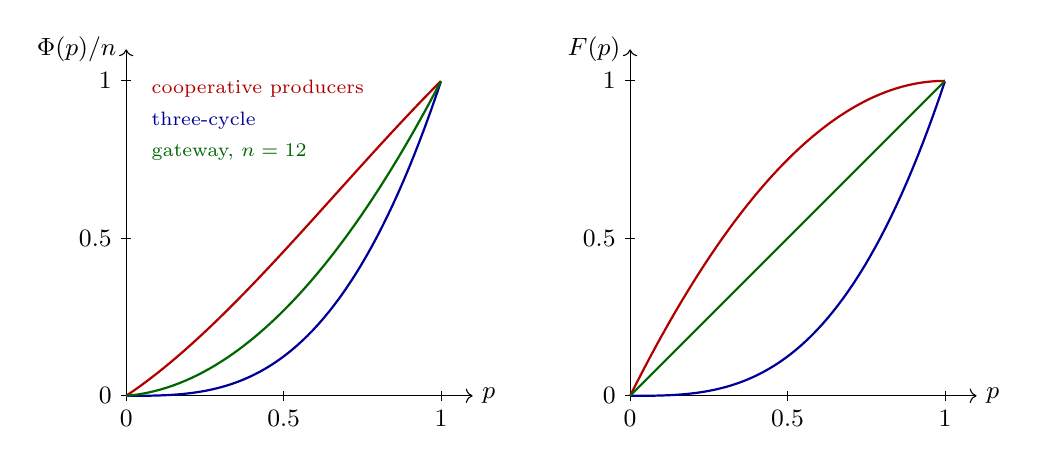
\begin{tikzpicture}[font=\small,scale=1]
\begin{scope}
\draw[->] (0,0) -- (4.4,0) node[right] {$p$};
\draw[->] (0,0) -- (0,4.4) node[left] {$\Phi(p)/n$};
\foreach \t in {0,0.5,1}{\draw (\t*4,0.06) -- (\t*4,-0.06) node[below] {\t}; \draw (0.06,\t*4) -- (-0.06,\t*4) node[left] {\t};}
\draw[red!70!black,thick,domain=0:1,samples=60] plot ({4*\x},{4*(2*\x+2*\x*\x-\x*\x*\x)/3});
\draw[blue!60!black,thick,domain=0:1,samples=60] plot ({4*\x},{4*\x*\x*\x});
\draw[green!40!black,thick,domain=0:1,samples=60] plot ({4*\x},{4*(\x+11*\x*\x)/12});
\node[red!70!black,anchor=west,font=\scriptsize] at (0.2,3.9) {cooperative producers};
\node[blue!60!black,anchor=west,font=\scriptsize] at (0.2,3.5) {three-cycle};
\node[green!40!black,anchor=west,font=\scriptsize] at (0.2,3.1) {gateway, $n=12$};
\end{scope}
\begin{scope}[xshift=6.4cm]
\draw[->] (0,0) -- (4.4,0) node[right] {$p$};
\draw[->] (0,0) -- (0,4.4) node[left] {$F(p)$};
\foreach \t in {0,0.5,1}{\draw (\t*4,0.06) -- (\t*4,-0.06) node[below] {\t}; \draw (0.06,\t*4) -- (-0.06,\t*4) node[left] {\t};}
\draw[red!70!black,thick,domain=0:1,samples=60] plot ({4*\x},{4*(2*\x-\x*\x)});
\draw[blue!60!black,thick,domain=0:1,samples=60] plot ({4*\x},{4*\x*\x*\x});
\draw[green!40!black,thick,domain=0:1,samples=60] plot ({4*\x},{4*\x});
\end{scope}
\end{tikzpicture}
\caption{Exact robustness curves, not simulation traces. Left: expected surviving fraction for the two-producer cooperative source ($\Phi=2p+2p^{2}-p^{3}$ on three reactions), a catalytic three-cycle ($\Phi=3p^{3}$), and a $12$-reaction gateway ($\Phi=p+11p^{2}$). Right: probability of any RAF for the same sources ($2p-p^{2}$, $p^{3}$ and $p$). The gateway retains $F(p)=p$ at every size; size and nonempty survival are distinct observables.}
\label{fig:curves}
\end{figure}

\subsection{Discriminating computations}

An exact preflight exhausts all $27$ functional maps on three reactions and their one-site resolutions: $729$ external-cut classifications and $2187$ target-gain identities at $p\in\{1/4,1/2,3/4\}$, $81$ functional variance identities, curvature on all $343$ elementary three-reaction graphs with nonempty catalytic rows, and curvature on $40$ additional four-reaction sources with varying food dependencies evaluated on their actual maxima. The cooperative fixture gives curvature $-2$ and the three-cycle $18$; the nine candidate objectives in the selector fixture were checked against direct literal evaluation. All checks pass in rational arithmetic in $0.167$\,s. These computations discriminate the stated formulas; they do not replace the proofs. Three scope boundaries were established the same way: an added catalyst can create a new cycle (Figure~\ref{fig:newcycle}); with several ambiguous reactions, independent local choices need not be represented by two global parent maps; and nonfood reactants invalidate the orbit adapter although Lemma~\ref{lem:onesite} still applies.

\section{Formal verification}\label{sec:formal}

\begin{sloppypar}
All theorems marked formal below are compiled in Lean~4 \citep{demoura2021}, toolchain \lean{leanprover/lean4:v4.30.0}, against Mathlib \citep{mathlib2020} at the matching tagged release with a frozen manifest. Verification treats every warning as an error, rejects \lean{sorry} and admitted proofs, extracts the requested declaration signatures, records the axioms used, and stores SHA-256 hashes of the source, the compiled module and the declaration interface in a receipt. Standard logical axioms (\lean{propext}, \lean{Classical.choice}, \lean{Quot.sound}) are permitted; their use does not make the Python implementations verified programs.
\end{sloppypar}

\subsection{Architecture}

The development is organized in three namespaces over a common finite reaction-system library (\lean{RAF}) providing closure, pruning, \lean{evaluate} (the maximum RAF) and their monotonicity lemmas.
\begin{itemize}[leftmargin=1.5em]\raggedright
\item \lean{RAFQueryCompilation}: \lean{RankedWitness} (Definition~\ref{def:witness}, the decidable checker, Theorem~\ref{thm:retention}, Theorem~\ref{thm:localization}), \lean{RankedExistence} (Lemma~\ref{lem:existence}), \lean{ResidualRAF} (Theorem~\ref{thm:residual}), the closure and pruning certificate chain of Section~\ref{sec:checking}, \lean{HybridQuery} (exact fallback), the charged and budgeted evaluators, \lean{FamilyArithmeticRun} (packet refinement) and \lean{TerminalFamily} (Theorem~\ref{thm:family}).
\item \lean{RAFSupportSelection}: \lean{SelectedCone} and \lean{Objective}, \lean{PerfectQuery}, \lean{IntrinsicDependence}, \lean{OneLayerSource}, \lean{MeanSetCover} with \lean{Aggregator}, \lean{PortfolioBoundary}, \lean{PortfolioCoverage} and \lean{SourcePortfolio}, \lean{ExponentialPortfolio}, \lean{SharedWitnessObstruction}, \lean{ClosedSeed}.
\item \lean{RAFReactionCriticality}: \lean{LossClosure}, \lean{GeneralPivotality} and \lean{SecondOrder} (finite product-measure derivatives), \lean{RAFCurvature}, \lean{CatalystChoice}, \lean{FunctionalSource} and \lean{Main}, \lean{TargetCuts}, \lean{CatalystIntervention}, \lean{ExposureVariance}, \lean{FunctionalVariance}, \lean{ExposureConcentration}, \lean{CatalyticModules}, \lean{ModularSurvival}, \lean{ModuleSensitivity}, \lean{Gateway}.
\end{itemize}

\subsection{Concordance}

\begin{table}[htbp]
\centering\footnotesize
\renewcommand{\arraystretch}{1.08}
\begin{tabular}{@{}>{\raggedright\arraybackslash}p{0.30\linewidth}>{\raggedright\arraybackslash}p{0.66\linewidth}@{}}
\toprule
Result & Module and principal declarations \\
\midrule
\multicolumn{2}{@{}l}{\emph{Namespace} \lean{RAFQueryCompilation}} \\
Witness checker; Thm.~\ref{thm:retention}; Thm.~\ref{thm:localization} & \lean{RankedWitness}: \lean{checkRankedSupport\_sound}; \lean{ranked\_retained\_fixed}; \lean{ranked\_deletion\_localization} \\
Lemma~\ref{lem:existence} & \lean{RankedExistence}: \lean{supported\_ranked\_exists}; \lean{raf\_ranked\_exists} \\
Thm.~\ref{thm:residual} & \lean{ResidualRAF}: \lean{residual\_supported}; \lean{evaluate\_residual} \\
Thm.~\ref{thm:family} & \lean{TerminalFamily}: \lean{ModuleFamily.family\_terminal\_factor}; setup cap in \lean{FamilySetup.familySetupCap} \\
\midrule
\multicolumn{2}{@{}l}{\emph{Namespace} \lean{RAFSupportSelection}} \\
Prop.~\ref{prop:floor} & \lean{IntrinsicDependence}: \lean{expected\_cone\_decomposition} \\
Thm.~\ref{thm:perfect} & \lean{PerfectQuery}: \lean{perfect\_query\_certificate}; \lean{loss\_iff\_every\_certificate} \\
Thm.~\ref{thm:preorder}; Thm.~\ref{thm:synergy} & \lean{IntrinsicDependence}: \lean{indispensable\_transitive}; \lean{mutual\_indispensability\_equivalence}; \lean{synergy\_obstructs\_perfect\_singletons} \\
Example~\ref{ex:twoproducer} & \lean{SharedWitnessObstruction}: \lean{OneLayer.two\_producer\_gap}; \lean{OneLayer.balanced\_two\_producer\_certificate} \\
Thm.~\ref{thm:onelayer} & \lean{OneLayerSource}: \lean{OneLayer.automatic\_selector\_globally\_optimal} \\
Thm.~\ref{thm:setcover} & \lean{MeanSetCover}: \lean{Aggregator.mean\_selection\_iff\_set\_cover}; \lean{Aggregator.source\_baseline} \\
Thm.~\ref{thm:portfolio} & \lean{PortfolioBoundary}: \lean{portfolioQuery\_correct} \\
Thm.~\ref{thm:greedy} & \lean{SourcePortfolio}: \lean{source\_portfolio\_selection}; \lean{PortfolioCoverage}: \lean{greedyPortfolio\_guarantee} \\
Thm.~\ref{thm:exponential} & \lean{ExponentialPortfolio}: \lean{Paired.exponential\_lower\_bound}; \lean{Paired.full\_portfolio\_exact}; \lean{Paired.two\_certificates\_singletons} \\
Prop.~\ref{prop:closedseed} & \lean{ClosedSeed}: \lean{closed\_seed\_exact\_loss} \\
\midrule
\multicolumn{2}{@{}l}{\emph{Namespace} \lean{RAFReactionCriticality}} \\
Prop.~\ref{prop:lossclosure}; Prop.~\ref{prop:firstorder} & \lean{LossClosure}: \lean{loss\_idempotent}; \lean{singleton\_loss\_nested}; \lean{GeneralPivotality}: \lean{size\_endpoint}; \lean{survival\_endpoint} \\
Thm.~\ref{thm:curvature} & \lean{SecondOrder}: \lean{second\_endpoint}; \lean{RAFCurvature}: \lean{raf\_second\_endpoint} (ordered-pair form) \\
Lemma~\ref{lem:onesite} & \lean{CatalystChoice}: \lean{evaluate\_one\_site\_choice} \\
Thm.~\ref{thm:exposure} & \lean{FunctionalSource}: \lean{evaluate\_iff\_orbit}; \lean{Main}: \lean{redundant\_orbit\_law}; \lean{redundant\_target\_probability} \\
Thm.~\ref{thm:cuts} & \lean{TargetCuts}: \lean{classification}; \lean{loss\_iff\_cut} \\
Thm.~\ref{thm:gain} & \lean{CatalystIntervention}: \lean{intervention\_gain}; \lean{total\_intervention\_gain}; \lean{singleton\_vulnerability\_reduction} \\
Thm.~\ref{thm:variance}; Cor.~\ref{cor:concentration} & \lean{ExposureVariance}: \lean{exposure\_variance}; \lean{FunctionalVariance}: \lean{functional\_variance}; \lean{normalized\_concentration}; \lean{ExposureConcentration}: \lean{exposure\_bounds} \\
Prop.~\ref{prop:modules} & \lean{CatalyticModules}: \lean{singleton\_loss}; \lean{mean\_size}; \lean{size\_bias\_probability}; \lean{ModularSurvival}: \lean{survival\_probability}; \lean{ModuleSensitivity}: \lean{mean\_derivative\_one} \\
Prop.~\ref{prop:gateway} & \lean{Gateway}: \lean{gateway\_nonempty\_iff}; \lean{gateway\_survival\_probability} \\
\bottomrule
\end{tabular}
\caption{Concordance between the results of this paper and the compiled declarations. Declaration names are given without their namespace prefix.}
\label{tab:concordance}
\end{table}

Table~\ref{tab:concordance} maps each result to its declarations. Some remarks on the formal statements. Perfect-query and intrinsic-dependence statements assume the baseline is a pruning fixed point; deletion sets are arbitrary finite sets, with reactions outside the baseline ignored by intersection with $S$. Source-specific statements instantiate literal reactant, product, food and catalyst data. The one-layer selector assumes nonempty allowed lists and natural weights; rational distributions reduce to this by scaling. The greedy theorem assumes a nonempty finite valid pool and $b\ge1$, and proves the cardinality bound, exactness for every $K$, and the coverage inequality against every $\mathcal B\subseteq H$ of size at most $b$. The derivative statements are \lean{HasDerivAt} facts about finite product-measure polynomials; the second-order statement counts ordered pairs, which is the factor two.

\subsection{What is proved by hand}\label{sec:notformal}

The following consequences are proved in this paper and not separately claimed as Lean declarations: the polynomial encoding and NP membership in Theorem~\ref{thm:npc}; the Taylor remainder in Corollary~\ref{cor:taylor}; the Chebyshev step in Corollary~\ref{cor:concentration}; the minimum-cardinality cases following Theorem~\ref{thm:cuts}; the strict-positivity criterion in Theorem~\ref{thm:gain}; the closed-form variances and the size-bias reading in Propositions~\ref{prop:modules} and~\ref{prop:gateway}; the numerical bookkeeping in the proof sketch of Theorem~\ref{thm:family}, which is however contained in the formal proof through the executable tariffs. The general Python witness proposer is checked by small independent oracles, not by an implementation-refinement theorem; the one-layer and finite-pool selectors have their own compiled contracts.

\section{Discussion}\label{sec:discussion}

\subsection{What the three parts say together}

The results separate three things that are easily conflated: the structural loss $L(K)$, the witness used to localize it, and the computation that certifies the answer. The loss is intrinsic: it is what every witness agrees on (Theorem~\ref{thm:perfect}), it induces a preorder on the baseline (Theorem~\ref{thm:preorder}), and its first and second moments under random deletion are exact functions of singleton and pair losses (Proposition~\ref{prop:firstorder}, Theorem~\ref{thm:curvature}). The witness is a choice: it can be optimized exactly on separable classes, it is NP-hard to optimize in general because a downstream aggregator makes shared ancestry observable, and no single witness can be perfect when losses are synergistic. The computation is exact whatever the witness, with a cost that is the region size plus boundary and certificate work, and with an unbounded structural amortization factor in a declared charge model but a measured break-even that depends on cold costs and workload length.

On the functional one-site class, the two exposures give a complete answer: shared exposure predicts singleton vulnerability, exclusive exposure identifies genuinely protective redundancy, and pairwise unions control joint fluctuations. Outside that class the curvature identity remains valid and separates overlap from cooperation, a distinction invisible to the mean singleton loss.

\subsection{Relation to incremental maintenance}

Delete/rederive \citep{gupta1993} and backward/forward maintenance \citep{motik2015} recover a materialization after deletion by over-deleting the derivations that used a deleted fact and rederiving what survives through alternative derivations. The ranked support witness plays the role of a stored derivation, and the cone is the over-deletion region; the residual solve is the rederivation. Two differences are specific to RAFs. The fixed point is a least closure nested inside a greatest pruning, so rederivation must handle the pruning of reactions whose catalysts disappear; and the catalytic parent is exempt from the rank order, so the stored derivation is not a proof tree. Theorem~\ref{thm:retention} is the statement that the retained part is nonetheless stable, and Theorem~\ref{thm:exponential} is a representation-size result of the kind studied in knowledge compilation \citep{darwiche2002}: singleton queries are cheap to compile and arbitrary deletion queries are not.

\subsection{Limitations and open problems}

\begin{itemize}
\item \emph{Source classes.} The exposure laws assume elementary food generation, private products and one alternative catalytic site. Several ambiguous sites, or nonfood reactants, need a new source-derived witness structure. Lemma~\ref{lem:onesite} is the only part that transfers unchanged.
\item \emph{Selection.} The NP-completeness concerns the uniform-mean objective. The worst-singleton objective, the complexity of the two-producer discriminator's minimax value on general sources, and approximation algorithms with guarantees relative to the intrinsic floor are open. Whether a bounded-arity aggregator recovers the exponential wall of Theorem~\ref{thm:exponential} is open.
\item \emph{Amortization.} Theorem~\ref{thm:family} compares with a specified fresh evaluator in a charge model. A theorem against every algorithm for a natural workload, or an amortized bound on a family with nontrivial regions, would be substantially stronger.
\item \emph{Biology.} No biological network was analysed. The deletion analysis of \citep{sousa2015} removes molecules as well as reactions and requires an explicit adapter; the present results are the structural and computational groundwork for such an analysis, not a substitute for it.
\item \emph{Kinetics.} None of the results assert kinetic persistence, positive steady states or thermodynamic feasibility of the surviving set.
\end{itemize}

\subsection{Reproducibility}

The Lean sources are in \lean{proofs/RAFQueryCompilation}, \lean{proofs/RAFSupportSelection} and \lean{proofs/RAFReactionCriticality}; each module has a strict verification receipt recording the toolchain, the manifest hash, the requested declarations, their interfaces and the axioms used. The preflight scripts and raw measurement outputs accompany the corresponding workspaces: the functional-source preflight and the selector comparison for Section~\ref{sec:robustness}; the held-out profiles, closed-seed discriminator, native selector check and stage-cost audit for Section~\ref{sec:selection}; the profile-frontier and cold-profile reports, with saved packets and exact mismatch assertions, for Section~\ref{sec:localization}. Every measurement is a single observation or a median over distinct source instances; no query is repeated to manufacture amortization. Source hashes distinguish instances.

\section*{Acknowledgements}
To be added.

\bibliographystyle{unsrtnat}
\bibliography{refs}

\end{document}
